\documentclass[border=10pt]{standalone}
\usepackage{tikz}
\usetikzlibrary{arrows.meta,shapes,calc}

\begin{document}
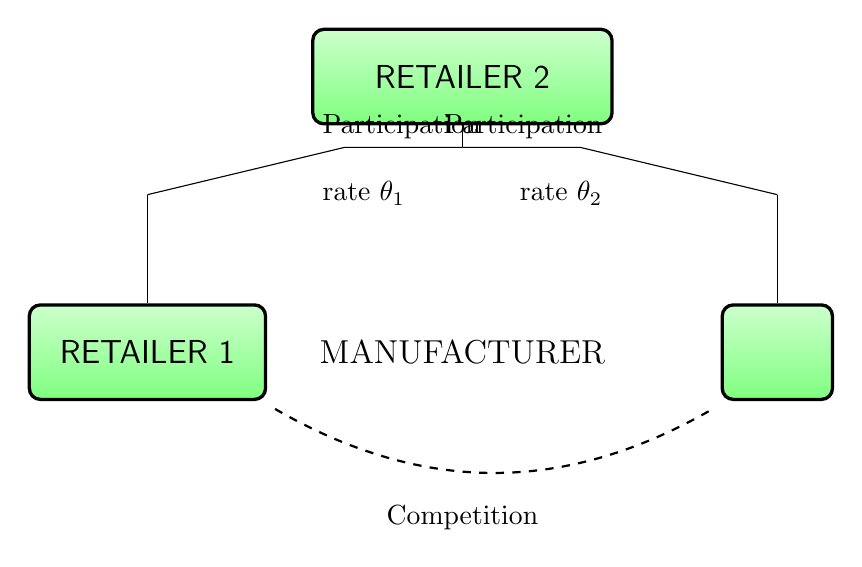
\begin{tikzpicture}[font=\sffamily]

% Styles
\tikzset{
  retailer/.style={
    draw,
    rounded corners=4pt,
    minimum width=3cm,
    minimum height=1.2cm,
    top color=green!20,
    bottom color=green!50,
    very thick
  },
  retailerSmall/.style={
    retailer,
    minimum width=1.4cm
  }
}

% Coordinates
\coordinate (M) at (0,0);
\coordinate (R1) at (-4,0);
\coordinate (R3) at (4,0); % right lower retailer (unnamed)
\coordinate (R2) at (0,3.5);

% Nodes
\node[retailer] (ret1) at (R1) {\large RETAILER 1};
\node[retailerSmall] (ret3) at (R3) {};
\node[retailer, minimum width=3.8cm] (ret2) at (R2) {\large RETAILER 2};

\node[font=\large] at (M) {MANUFACTURER};

% Vertical and horizontal connecting lines from RETAILER 2
% center down from RETAILER 2
\coordinate (midTop) at ($(R2)+(0,-0.9)$);
\draw (ret2.south) -- (midTop);

% to left retailer
\coordinate (leftTop) at (-4,2.0);
\draw (midTop) -- ++(-1.5,0) coordinate (midLeft) -- (leftTop);
\draw (leftTop) -- (ret1.north);

% to right retailer
\coordinate (rightTop) at (4,2.0);
\draw (midTop) -- ++(1.5,0) coordinate (midRight) -- (rightTop);
\draw (rightTop) -- (ret3.north);

% Participation labels
\node[anchor=south west, font=\normalsize] at ($(leftTop)!0.5!(ret2.south)+(0.1,0.15)$) {Participation};
\node[anchor=north west, font=\normalsize] at ($(leftTop)!0.5!(ret2.south)+(0.1,-0.15)$) {rate $\theta_1$};

\node[anchor=south east, font=\normalsize] at ($(rightTop)!0.5!(ret2.south)+(-0.1,0.15)$) {Participation};
\node[anchor=north east, font=\normalsize] at ($(rightTop)!0.5!(ret2.south)+(-0.1,-0.15)$) {rate $\theta_2$};

% Competition dashed arc between lower retailers
\draw[dashed, line width=0.8pt]
  ($(ret1.south east)+(0.1,-0.1)$)
  to[out=-30,in=-150]
  ($(ret3.south west)+(-0.1,-0.1)$);

\node[font=\normalsize] at (0,-2.1) {Competition};

\end{tikzpicture}
\end{document}